%-------------------------------------------------------
%-- PREAMBLE
%-------------------------------------------------------
\documentclass[a4paper,10pt]{article} % Uses article class in A4 format

% Includes preamble configurations
% --------------------------------------------------------------------
% Packages
% --------------------------------------------------------------------
\usepackage[a4paper, margin=1.5cm]{geometry}

% Text, input, language-related packages
\usepackage[utf8]{inputenc}
\usepackage[T1]{fontenc}
\usepackage[english]{babel}
\usepackage[protrusion=true,expansion=true]{microtype} 

% Math packages
\usepackage{amsmath,amsfonts,amsthm,amssymb,bm,mathdots,mathtools,bigints}

% TiKz packages
\usepackage{tikz, pgfplots, tikzsymbols, tikzducks}

% Graphic and color packages
\usepackage[export]{adjustbox}				% Environment to adjust LaTeX objects
\usepackage[skins]{tcolorbox}				% Coloured boxes for LaTeX objects
\usepackage{graphicx} 						% Enhanced support for graphics
\usepackage{color, xcolor}					% Driver-independent color extensions
\usepackage{wrapfig}						% Environment to wrap figures/tables
\usepackage{subcaption}						% Environment to create subcaptions

% General utilities
\usepackage[nodayofweek]{datetime}			% Customize date commands
\usepackage[printwatermark]{xwatermark}		% Watermarks the document
\usepackage[document]{ragged2e}				% Text-alignment (\centering, ...)
\usepackage{stfloats}						% Control presentation of floats
\usepackage{framed, mdframed}				% Framed and shaded environments
\usepackage{multicol}						% Multicolumn environment
\usepackage{environ}						% Better interface for environments
\usepackage{minted, listings}				% Coding environments
\usepackage{hyperref}				        % Support for hypertext and links
\usepackage{enumerate}				        % Options for enumerate environments
\usepackage{etoolbox}						% Environment hooks (\BeforeBegin...)
\usepackage{parskip}						% Manages paragraph spacing stuff
% --------------------------------------------------------------------
% Packages Configurations
% --------------------------------------------------------------------
% (general): Define general paragraphing spaces and mono font
\setlength{\parskip}{0cm}
\setlength{\parindent}{0cm}

% (tikz): Imports some custom libraries and pgfplot settings
\usetikzlibrary{shapes, arrows, decorations.pathmorphing}
\usetikzlibrary{backgrounds, positioning, fit, calc}
\usetikzlibrary{bayesnet, graphs}

\pgfplotsset{compat=1.16} 

% (minted): Set styling configurations
\usemintedstyle{pastie}
\setminted{ linenos=true,             % Line numbers
            autogobble=true,          % Automatically remove common white space
            frame=lines,
            framesep=2mm}

\renewcommand{\theFancyVerbLine}{\sffamily {\normalsize \oldstylenums{\arabic{FancyVerbLine}}}}

% (listings): Defines the code styling and formatting
\lstset{
    backgroundcolor=\color[RGB]{39,40,34},
    language=matlab, keywordstyle=\color[RGB]{102,217,239},
    basicstyle=\footnotesize \ttfamily,breaklines=true,
    escapeinside={\%*}{*)}
}

% (datetime): Personalized date commands (apply them before a \today)
\newdateformat{datenum}{\twodigit{\THEDAY}/\twodigit{\THEMONTH}/\THEYEAR}
\newdateformat{datefull}{\twodigit{\THEDAY}{ }\monthname[\THEMONTH], \THEYEAR}

% (hyperref): Setup link colors and other properties
\hypersetup{
    colorlinks=true,
    linkcolor=black!95!white,
    filecolor=magenta,      
    urlcolor=cyan,
}


% --------------------------------------------------------------------
% Other Definitions
% --------------------------------------------------------------------
% Additional cool colors
\definecolor{stateColor}{cmyk}{0.82,0,0.92,0}
\definecolor{inputColor}{RGB}{73,158,255}
\definecolor{disturbanceColor}{RGB}{102,43,153}
\definecolor{outputColor}{RGB}{224,60,48}

% --------------------------------------------------------------------
% Commands
% --------------------------------------------------------------------

% A light title-page header
\newcommand*{\thetitle}{%
    \vskip0.5cm%
    \begin{minipage}{0.3\textwidth} % Left side of title section
        \raggedright
        \institute\\\course\\[0.5ex]\footnotesize\professor
        \medskip\hrule
    \end{minipage}\hfill
    \begin{minipage}{0.4\textwidth} % Center of title section
        \centering 
        {\huge \bfseries Homework \assnumber}\\[1ex]{\LARGE\title}\\
    \end{minipage}\hfill
    \begin{minipage}{0.3\textwidth} % Right side of title section
        \raggedleft
        {\author$\ $(\authorid)}\\\texttt{(\email)}\\[0.5ex]\footnotesize\today
        \medskip\hrule
    \end{minipage}
    \vskip1cm 
}

% Colored hyperlinks
\newcommand{\chref}[2]{
  \href{#1}{{\usebeamercolor[bg]{Feather}#2}}
}

% A cooler transpose symbol 'T'
\newcommand*{\tran}{{\mkern-1.5mu\mathsf{T}}}

% Cool tensor sub- and super-scripts (\tend and \tenq, respectively)
\newcommand{\tend}[1]{\hbox{\oalign{$\bm{#1}$\crcr\hidewidth$\scriptscriptstyle\bm{\sim}$\hidewidth}}}
\newcommand{\tenq}[1]{\hbox{\oalign{$\bm{#1}$\crcr\hidewidth$\scriptscriptstyle\bm{\sim}$\hidewidth}}}

% Argmax and Argmin math operators
\DeclareMathOperator*{\argmax}{arg\,max}
\DeclareMathOperator*{\argmin}{arg\,min}

% --------------------------------------------------------------------
% Environments
% --------------------------------------------------------------------

% Boxed-enviroment with counter for each problem
\newcounter{problem}
\makeatletter
\newenvironment{problem}
    {%
    \refstepcounter{problem} \begin{tcolorbox}[
    fuzzy shadow={0.2mm}{-0.2mm}{0mm}{0.1mm}{black!50!white},
    enhanced, shrink tight, 
    extrude by=3mm, 
    colframe=black,
    colback=black!5!white,
    arc=1pt,
    boxrule=0.5pt]
    {\bf Problem~\theproblem.}%
    }%
    {%
    \end{tcolorbox}\vskip0.5cm
    }

% Simple solution environment with end square
\makeatletter
\newenvironment{solution}
    {%
    {\bf Solution.}%
    }%
    {%
    \hfill$\square$
    }%

% Wrapper for the minted environment
\makeatletter
\newenvironment{code}[3][0.8\textwidth]
    {%
    \VerbatimEnvironment
    \begin{minipage}{\textwidth} \centering%
    \begin{minipage}{#1}%
    \begin{listing}[H]%
    \caption{#2}\label{#3}%
    \begin{minted}{julia}%
    }%
    {%
    \end{minted}
    \end{listing}%
    \end{minipage}%
    \end{minipage}%
    \vskip0.5cm
    }

% --------------------------------------------------------------------
% Unicode Characters Definition (for Julia Minted)
% --------------------------------------------------------------------
\DeclareUnicodeCharacter{3B4}{$\bm{\delta}$}
\DeclareUnicodeCharacter{3B8}{$\bm{\theta}$}
\DeclareUnicodeCharacter{3BB}{$\lambda$}
\DeclareUnicodeCharacter{3BC}{$\mu$}
\DeclareUnicodeCharacter{3BC}{$\pi$}
\DeclareUnicodeCharacter{3C3}{$\sigma$}
\DeclareUnicodeCharacter{3C0}{$\pi$}
\DeclareUnicodeCharacter{3D5}{$\bm{\phi}$}
\DeclareUnicodeCharacter{2208}{$\in$}
\DeclareUnicodeCharacter{2297}{$\otimes$}
\DeclareUnicodeCharacter{2A02}{$\bigotimes$}
\DeclareUnicodeCharacter{2299}{$\odot$}
\DeclareUnicodeCharacter{22C4}{$\diamond$}
\DeclareUnicodeCharacter{209A}{$_{p}$}
\DeclareUnicodeCharacter{221A}{$\sqrt{}$}
\DeclareUnicodeCharacter{2248}{$\approx$}
\DeclareUnicodeCharacter{2080}{$_o$}
\DeclareUnicodeCharacter{2090}{$_a$}
\DeclareUnicodeCharacter{03B1}{$\alpha$}
\DeclareUnicodeCharacter{1D65}{$_v$}
\DeclareUnicodeCharacter{2096}{$_k$}
\DeclareUnicodeCharacter{1D63}{$_r$}
\DeclareUnicodeCharacter{2081}{$_1$}
\DeclareUnicodeCharacter{2082}{$_2$}
\DeclareUnicodeCharacter{2083}{$_3$}
\DeclareUnicodeCharacter{2084}{$_4$}
\DeclareUnicodeCharacter{208C}{$_=$}
\DeclareUnicodeCharacter{208B}{$_-$}
\DeclareUnicodeCharacter{208A}{$_+$}
\DeclareUnicodeCharacter{2211}{$\Sigma$}
\DeclareUnicodeCharacter{03A3}{$\Sigma$}
\DeclareUnicodeCharacter{03A0}{$\Pi$}
\DeclareUnicodeCharacter{1D4E7}{$\mathcal{X}$}
\DeclareUnicodeCharacter{2093}{$_x$}
\DeclareUnicodeCharacter{1D67}{$_y$}
\DeclareUnicodeCharacter{2260}{$\neq$}
\DeclareUnicodeCharacter{208D}{$_($}
\DeclareUnicodeCharacter{2099}{$_n$}
\DeclareUnicodeCharacter{2C7C}{$_i$}
\DeclareUnicodeCharacter{209C}{$_t$}
\DeclareUnicodeCharacter{208E}{$_)$}
\DeclareUnicodeCharacter{1D4E8}{$\mathcal{Y}$}
\DeclareUnicodeCharacter{2A09}{$\times$}
\DeclareUnicodeCharacter{207D}{$^($}
\DeclareUnicodeCharacter{2074}{$^4$}
\DeclareUnicodeCharacter{2075}{$^5$}
\DeclareUnicodeCharacter{207F}{$^n$}
\DeclareUnicodeCharacter{1D48}{$^d$}
\DeclareUnicodeCharacter{1D3A}{$^N$}
\DeclareUnicodeCharacter{1D34}{$^H$}
\DeclareUnicodeCharacter{207E}{$^)$}
\DeclareUnicodeCharacter{207B}{$^-$}
\DeclareUnicodeCharacter{207A}{$^+$}
\DeclareUnicodeCharacter{1D4E2}{$\mathcal{S}$}
\DeclareUnicodeCharacter{1D4E4}{$\mathcal{U}$}
\DeclareUnicodeCharacter{1D40}{$^T$}
\DeclareUnicodeCharacter{03F5}{$\epsilon$}
\DeclareUnicodeCharacter{022EF}{$\cdots$}
\DeclareUnicodeCharacter{1D62}{$_i$}
\DeclareUnicodeCharacter{2218}{$\circ$}
\DeclareUnicodeCharacter{1D4E5}{$\mathcal{V}$}
\DeclareUnicodeCharacter{1D4D8}{$\mathcal{I}$}
\DeclareUnicodeCharacter{1D4D0}{$\mathcal{A}$}
\DeclareUnicodeCharacter{1D4D6}{$\mathcal{G}$}
\DeclareUnicodeCharacter{211D}{$\mathbb{R}$}

% --------------------------------------------------------------------

% --------------------------------------------------------------------
% *************************** FRONT MATTER ***************************
% --------------------------------------------------------------------
\def\assnumber{12}
\def\title{Tensor Train Singular Value Decomposition (TTSVD)}
\def\author{Otacílio B. L. Neto}
\def\authorid{481736}
\def\email{minhotmog@alu.ufc.br}
\def\institute{Universidade Federal do Ceará}
\def\course{TIP8419 - Tensor Algebra}
\def\professor{Prof. André A., Prof. Maryam D.} 

% ====================================================================

% --------------------------------------------------------------------
% ***************************** DOCUMENT *****************************
% --------------------------------------------------------------------
\begin{document} \sloppy

%-------------------------------------------------------
% TITLE PAGE
%-------------------------------------------------------
\thetitle

%-------------------------------------------------------
% PROBLEM 1
%-------------------------------------------------------
\vskip-0.4cm
\begin{problem} \justifying
We will go to implement the TT-SVD (Tensor Train Singular Value Decomposition) algorithm. The TT Decomposition of a $N$-order tensor $\mathcal{X} \in \mathbb{R}^{I_1\times I_2 \times \cdots \times I_N}$, with TT-Ranks ($R_1, R_2, \cdots, R_{N-1}$), is a decomposition of the tensor $\mathcal{X}$ into a train of tensors as 
\begin{equation*}
    \mathcal{X} = \mathbf{G}_1 \times_2^1 \mathcal{G}_2 \times_3^1 \mathcal{G}_3  \times_4^1 \cdots \times_{N-1}^1 \mathcal{G}_{N-1} \times_{N}^1 \mathbf{G}_N.
\end{equation*}

\noindent For a $4$-order tensor $\mathcal{X} \in \mathbb{R}^{5\times 5\times 5\times 5}$, implement the TT-SVD algorithm to estimate the TT-cores $\mathbf{G}_1 \in \mathbb{C}^{5\times R_1}$, $\mathcal{G}_2 \in \mathbb{C}^{R_{1}\times 5\times R_2}$, $\mathcal{G}_3 \in \mathbb{C}^{R_{2}\times 5\times R_3}$, and $\mathbf{G}_4 \in \mathbb{C}^{R_3 \times 5}$ that forms the TT Decomposition of $\mathcal{X}$, for given ranks ($R_1,R_2,R_3$). For randomly generated ($\mathbf{G}_1, \mathcal{G}_2, \mathcal{G}_3, \mathbf{G}_4$), compare the original tensor $\mathcal{X}$ with the one reconstructed by the TT-SVD.

\end{problem}

\begin{solution} \justifying

\noindent The function is implemented in Julia (v1.4), and is shown in Listing \ref{lst: code1}.  Regarding the present implementation, lines 2--14 define an auxiliary function to compute the tensor train products. The Train Tensor Singular Value Decomposition (TT-SVD) algorithm is then implemented in lines 17--237, following the pseudocode provided in the course material. 

\begin{code}[0.95\textwidth]{The Tensor-Train Singular Value Decomposition (TTSVD) algorithm for Problem 1.}{lst: code1}
# ==== FUNCTIONS ====
# The Tensor-Train product function
function ×¹(G...)
    # Auxiliary variables with dimension/rank information
    IR  = [size(G[1]); [size(G[i])[2:end] for i=2:length(G)]...]
    I,R = ([IR[i][1] for i=1:length(G)], [IR[i][2] for i=1:length(G)-1])
    
    # Tensor-train product loop
    𝓧 = zeros(I...)
    for i in CartesianIndices(𝓧), r in CartesianIndices((R[1],R[2],R[3]))
        𝓧[i] += G[1][i[1],r[1]]*G[2][r[1],i[2],r[2]]*G[3][r[2],i[3],r[3]]*G[4][r[3],i[4]]
    end
    return 𝓧    # Returns the resulting tensor
end

# The Tensor-Train Singular Value Decomposition (TTSVD) algorithm
function TTSVD(𝓧)
    I = size(𝓧)                                     # Auxiliary variable
                                                    #
    X¹ = reshape(𝓧, (I[1],Π(I[2:4])))               # Unfolds the tensor [𝓧]₁ ∈ ℝ(I₁,I₂I₃I₄)
    U,Σ,V = svd(X¹);    Σ = Diagonal(Σ);            # Computes the SVD [𝓧]₁ = UΣVᴴ
    R₁ = sum(diag(Σ) .> 1e-6)                       # Gets the number of nonzero singular-values
    U₁ = U[:,1:R₁];  V₁ = (Σ*(V)ᴴ)[1:R₁,:]          # Truncates pair (U,V) given R₁
    G₁ = U₁                                         # Stores the 1st factor G₁ ∈ ℝ(I₁,R₁)
                                                    #
    X² = reshape(V₁, (R₁*I[2], Π(I[3:4])))          # Unfolds the matrix X² = [V₁]₁ ∈ ℝ(R₁I₂,I₃I₄)
    U,Σ,V = svd(X²);    Σ = Diagonal(Σ);            # Computes the SVD X² = UΣVᴴ
    R₂ = sum(diag(Σ) .> 1e-6)                       # Gets the number of nonzero singular-values
    U₂ = U[:,1:R₂];  V₂ = (Σ*(V)ᴴ)[1:R₂,:]          # Truncates pair (U,V) given R₂
    𝓖₂ = reshape(U₂, (R₁, I[2], R₂))                # Reshapes the 2nd factor 𝓖₂ ∈ ℝ(R₁,I₂,R₂)
                                                    # 
    X³ = reshape(V₂, (R₂*I[3], I[4]))               # Unfolds the matrix X³ = [V₂]₁ ∈ ℝ(R₂I₃,I₄)
    U,Σ,V = svd(X³);    Σ = Diagonal(Σ);            # Computes the SVD X³ = UΣVᴴ
    R₃ = sum(diag(Σ) .> 1e-6)                       # Gets the number of nonzero singular-values
    U₃ = U[:,1:R₃];  V₃ = (Σ*(V)ᴴ)[1:R₃,:]          # Truncates pair (U,V) given R₃
    𝓖₃ = reshape(U₃, (R₂, I[3], R₃))                # Reshapes the 3rd factor 𝓖₃ ∈ ℝ(R₂,I₃,R₃)
    G₄ = V₃[1:R₃,:]                                 # Stores the 4th factor G₄ ∈ ℝ(R₃,I₄)

    return (G₁, 𝓖₂, 𝓖₃, G₄)                         # Returns the decomposition factors
end
    
\end{code} 

The function $\times^1(\cdot)$ implements the element-wise TT decomposition through the formula
$$
    x_{i_1,i_2,\cdots,i_N} = \sum_{r_1 = 1}^{R_1} \sum_{r_2 = 1}^{R_2} \sum_{r_3 = 1}^{R_3} \cdots \sum_{r_{N-2} = 1}^{R_{N-2}} \sum_{r_{N-1} = 1}^{R_{N-1}} \mathbf{G}_{1_{i_1,r_1}} \mathcal{G}_{2_{r_1,i_2,r_2}} \mathcal{G}_{3_{r_2,i_3,r_3}} \cdots \mathcal{G}_{{N-1}_{r_{N-2},i_{N-1},r_{N-1}}} \mathbf{G}_{N_{r_N,i_{N-1}}}.
$$
The TT-SVD algorithm follows the procedure described by the tensor network shown in Fig. \ref{fig: f1}

\begin{figure}[ht] \centering
    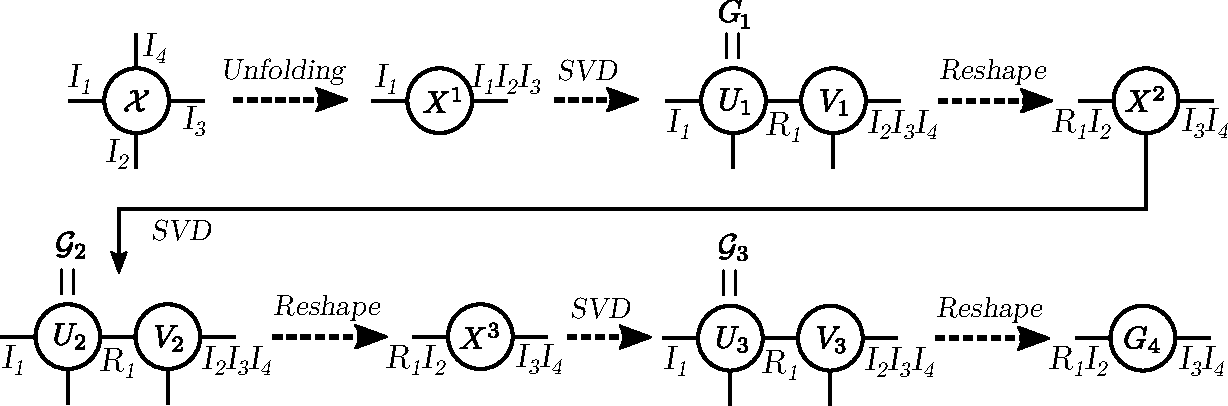
\includegraphics[width=0.9\textwidth]{imgs/TensorNetwork.pdf}
    \caption{Illustration of the TT-SVD algorithm using a Tensor Network framework.}
    \label{fig: f1}
\end{figure}

The implementation is tested through the script presented at Listing \ref{lst: code2}.
The execution of the assertion tests at lines 10 and 18 do not result in any failed assertion, thus indicating that the function outputs the expected results for the given tests. Specifically, executing lines 11 and 19 shows that, on average, $\| \mathcal{X} - \hat{\mathcal{X}} \|_F^2 \approx 1.2\cdot10^{-26}$ for $\hat{\mathcal{X}} = \hat{\mathbf{G}}_1 \times_2^1 \hat{\mathcal{G}}_2 \times_3^1 \hat{\mathcal{G}}_{3} \times_{4}^1 \hat{\mathbf{G}}_4$ with all TT-cores obtained from the TT-SVD. Thus, it is possible to conclude that factors $(\hat{\mathbf{G}}_1, \hat{\mathcal{G}}_2, \hat{\mathcal{G}}_3, \hat{\mathbf{G}}_4)$ comprise a valid decomposition of the original tensor $\mathcal{X}$. 

\begin{code}[0.9\textwidth]{Script used to test the TTSVD algorithm implementation.}{lst: code2}
# ==== SCRIPT ====
# -- Case 1: Generating 𝓧 from factors (G₁, 𝓖₂, 𝓖₃, G₄) --
# Randomly generates the TT factors and computes the tensor 𝓧 = G₁ ×¹ 𝓖₂ ×¹ 𝓖₃ ×¹ G₄
R = [4 3 4];     # Ranks used for the decomposition
G₁ = randn(5,R[1]); 𝓖₂ = randn(R[1],5,R[2]); 𝓖₃ = randn(R[2],5,R[3]); G₄ = randn(R[3],5);
𝓧 = ×¹(G₁, 𝓖₂, 𝓖₃, G₄);

G₁_, 𝓖₂_, 𝓖₃_, G₄_ = TTSVD(𝓧);      # Estimates the factors (G₁, 𝓖₂, 𝓖₃, G₄)

@assert 𝓧 ≈ ×¹(G₁_, 𝓖₂_, 𝓖₃_, G₄_)
@show norm(𝓧 - ×¹(G₁_, 𝓖₂_, 𝓖₃_, G₄_))^2

# -- Case 2: Directly generating 𝓧 randomly --
𝓧 = randn(5, 5, 5, 5);

G₁_, 𝓖₂_, 𝓖₃_, G₄_ = TTSVD(𝓧);      # Estimates the factors (G₁, 𝓖₂, 𝓖₃, G₄)

@assert 𝓧 ≈ ×¹(G₁_, 𝓖₂_, 𝓖₃_, G₄_)
@show norm(𝓧 - ×¹(G₁_, 𝓖₂_, 𝓖₃_, G₄_))^2

# ==== ====
\end{code} 

Moreover, we verified that the resulting estimated tensors $(\hat{\mathbf{G}}_1, \hat{\mathcal{G}}_2, \hat{\mathcal{G}}_3, \hat{\mathbf{G}}_4)$ are not actually good approximations of the original factors used to generate $\mathcal{X}$. In fact, we have average distances of 
$$
    \| \mathbf{G}_1 - \hat{\mathbf{G}}_1 \|_F^2 = 25.1,\ \ \  
    \| \mathcal{G}_2 - \hat{\mathcal{G}}_2 \|_F^2 = 61.7,\ \ \ 
    \| \mathcal{G}_3 - \hat{\mathcal{G}}_3 \|_F^2 = 62.6,\ \ \ 
    \| \mathbf{G}_4 - \hat{\mathbf{G}}_4 \|_F^2 = 3\cdot 10^4. 
$$
This result is expected, since the decomposition is not unique: is always possible to replace a pair of successive TT-cores $\mathcal{G}_j$ and $\mathcal{G}_{j+1}$ by $\tilde{\mathcal{G}}_j = \mathcal{G}_j \times_{3}^1 \mathbf{M}_j^{-1}$ and $\tilde{\mathcal{G}}_{j+1} = \mathbf{M}_j \times_{2}^1 \mathcal{G}_{j+1}$ without changing the resulting tensor $\mathcal{X}$.

\end{solution}
\vskip0.5cm

%-------------------------------------------------------
\end{document}
